%% ------------------------------------------------------------------------------------------- Introduction
\section{Introduction}
\label{sec:intro}

Many universities take attendance by projecting a QR code. The code is easy to forward: a student in the room
photographs it and sends it to an absent friend. Rotating the code every few seconds narrows that window but does
not prove \emph{who} scanned it. Our system adds two checks to a 3\,s rotating QR code. After scanning, the phone
shows a \emph{random hand gesture} (one of five HaGRID~\cite{hagrid} classes). The student takes a selfie showing
that gesture next to their face, and the server accepts the check-in only if
(i) the recognised gesture equals the challenge (a challenge--response liveness test~\cite{iso30107}) and
(ii) the face matches the student's enrolled ArcFace~\cite{arcface} embedding.

The vision problem is recognising the gesture reliably in a phone photo. Gesture detectors work on a downscaled
copy of the whole frame (MediaPipe's palm detector sees 192\,px~\cite{mphands}, YOLO~\cite{yolov8} 640\,px), so a
hand that covers a few percent of a 12\,MP selfie is reduced to a few pixels. Classmates in the background also
raise hands, and a full-frame detector cannot tell whose hand it sees.
Our \textbf{contribution} is a \emph{face-anchored ROI cascade}: a face detector (BlazeFace~\cite{blazeface} or
SCRFD~\cite{scrfd}) finds the selfie-taker's face, a window of $s\times$ the face box is cut out at native
resolution, and the \emph{same} gesture detector runs on this up-scaled crop. The crop gives the hand more pixels
and ties the gesture to the face that is verified. We test it in a paired comparison with the same detector on
the same 2,400 held-out images, ablate the ROI size and the anchor, and report where it fails.

\noindent\textbf{Hypothesis (H1).} With the same detector, the cascade raises top-1 gesture accuracy by
$\geq$5 percentage points (pp) over full-frame inference on held-out subjects, at $\leq$50\,ms extra CPU latency.

\noindent\textbf{Related work.} Using one detection to crop the input of a second model is a classic idea, from
boosted cascades~\cite{violajones} to hand keypoint estimators that crop hands from body keypoints~\cite{simon2017hand}
and MediaPipe's palm-detector$\rightarrow$landmark pipeline~\cite{mphands,mediapipe}. Slicing small-object
detectors into tiles (SAHI~\cite{sahi}) also trades extra detector calls for resolution. We use the \emph{face}
as the anchor. The face is needed for identity anyway, so the cascade adds one detector call, not $k$ tiles. We
evaluate on HaGRID~\cite{hagrid,hagridv2}, the largest public static-gesture dataset. Its subjects record
selfie-like images, and it provides a subject-disjoint split.

%% ------------------------------------------------------------------------------------------- Method
\section{Method}
\label{sec:method}

\begin{figure*}[t]
  \centering
  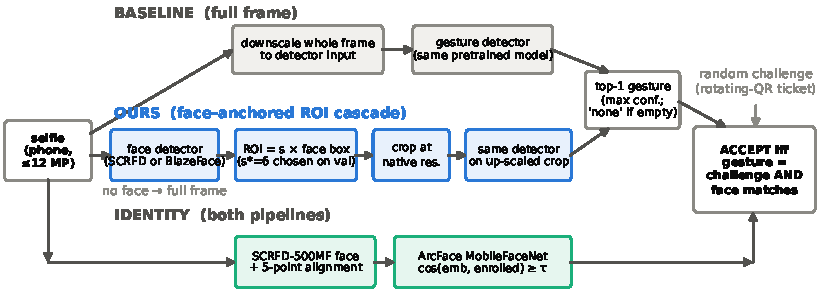
\includegraphics[width=0.92\linewidth]{figures/pipeline.pdf}
  \vspace{-2mm}
  \caption{\textbf{Pipeline.} Baseline (top): the gesture detector sees the whole, downscaled frame. Ours
  (middle): face detector $\rightarrow$ ROI $=s\times$ face box $\rightarrow$ the same detector on the crop. The
  detections are mapped back to image coordinates. Both pipelines share the identity branch (bottom) and the
  accept rule.}
  \label{fig:pipeline}
  \vspace{-3mm}
\end{figure*}

\noindent\textbf{Baseline.} The gesture detector runs on the full image. The predicted gesture is the class of
the highest-confidence detection, or \texttt{none} if there is no detection.

\noindent\textbf{Proposed cascade} (\cref{fig:pipeline}). (1)~A face detector finds faces, and the \emph{largest}
one is taken as the selfie-taker. The proposal used BlazeFace short-range (MediaPipe Tasks, conf.\ 0.5). We also
test SCRFD-500MF, which the identity branch runs anyway. (2)~The ROI is a box of $s\cdot w_f\times s\cdot h_f$
centred on the face, clipped to the image and rounded to whole pixels. The proposal fixed $s{=}3$; the final
system uses the anchor and $s$ chosen on the val split (\cref{sec:exp}). (3)~The crop is passed to the detector at
native resolution, so the detector's own resizing \emph{up-scales} small crops. (4)~Detections are shifted back by
the crop offset, and the top-1 rule is the same as the baseline's. If no face is found, the pipeline falls back to
the full frame. This fallback is counted and reported.

\noindent\textbf{Gesture detector.} Both pipelines use Google's \emph{pretrained} MediaPipe Gesture
Recognizer~\cite{mphands} (palm detector, 21 hand landmarks, gesture classifier), the same model the deployed app
uses. Its classes are mapped to five HaGRID gestures (like, peace, palm, fist, one; it has no ``ok''). We keep a
label only if its score is $\geq$0.5, and its box is the landmark extent. The detector was trained by a third
party, so neither pipeline has seen our data. The detector is an interchangeable module: the repository also
contains a YOLOv8n~\cite{yolov8} fine-tuning path (\texttt{train\_yolo.py}), which we did not evaluate for this
report.

\noindent\textbf{Identity.} SCRFD-500MF~\cite{scrfd} detects the face and its 5 landmarks. The face is aligned to
112$\times$112 and embedded by ArcFace MobileFaceNet~\cite{mobilefacenet,arcface} (InsightFace \texttt{buffalo\_s},
run with onnxruntime). A probe is accepted when its cosine similarity to the enrolled embedding is $\geq\tau$.
$\tau{=}\lfwThr$ maximises accuracy on LFW~\cite{lfw} DevTrain (DevTest: \lfwTestAcc\% accuracy, FAR
\lfwTestFAR\%, FRR \lfwTestFRR\%), with no training on our data.
